% XeLaTeX can use any Mac OS X font. See the setromanfont command below.
% Input to XeLaTeX is full Unicode, so Unicode characters can be typed directly into the source.

% The next lines tell TeXShop to typeset with xelatex, and to open and save the source with Unicode encoding.

%!TEX TS-program = xelatex
%!TEX encoding = UTF-8 Unicode

\documentclass[11pt]{article}

% See geometry.pdf to learn the layout options. There are lots.
\usepackage[papersize={8.5in,11in}, total={7in,9.5in},top=20mm, left=20mm, includefoot]{geometry}

\setlength{\parindent}{10pt}
\setlength{\parskip}{2pt}


\usepackage{graphicx}
\usepackage{amssymb}
\usepackage{etaremune}
%\bibliographystyle{natbib} % this must remain commented

\makeatletter
\long\def\thebibliography#1{%
  \section*{\refname}%
  \@mkboth{\MakeUppercase\refname}{\MakeUppercase\refname}
  \settowidth{\dimen0}{\@biblabel{#1}}%
  \setlength{\dimen2}{\dimen0}%
  \addtolength{\dimen2}{\labelsep}
  \sloppy
  \clubpenalty 4000 
  \@clubpenalty 
  \clubpenalty 
  \widowpenalty 4000
  \sfcode `\.\@m

  \renewcommand{\labelenumi}{\@biblabel{\theenumi}} % labels like [3], [2], [1]
  \begin{etaremune}[labelwidth=\dimen0,leftmargin=\dimen2]\@openbib@code
}
\def\endthebibliography{\end{etaremune}}
\def\@bibitem#1{%
  \item \if@filesw\immediate\write\@auxout{\string\bibcite{#1}{\the\value{enumi}}}\fi\ignorespaces
}
\makeatother
%\renewcommand\bibnumfmt[1]{\emph{\textbf{\small{#1)}}}}
%\usepackage{graphicx}[pdftex]
%\usepackage{wrapfig}
\usepackage{caption}
\linespread{1}
%\usepackage{setspace}
% Will Robertson's fontspec.sty can be used to simplify font choices.
% To experiment, open /Applications/Font Book to examine the fonts provided on Mac OS X,
% and change "Hoefler Text" to any of these choices.
\usepackage{xspace}
\usepackage{fontspec,xltxtra,xunicode}
\defaultfontfeatures{Mapping=tex-text}
\setromanfont[Mapping=tex-text]{Palatino}
\setsansfont[Scale=MatchLowercase,Mapping=tex-text]{Gill Sans}
\setmonofont[Scale=MatchLowercase]{Andale Mono}

%set the bibliography style
%\usepackage[super,sort&compress,comma]{natbib}
%%\bibliographystyle{unsrt}


%set up a header
\usepackage{fancyhdr}
\pagestyle{fancy}
\lhead{\textbf{GB Gloor}} \chead{\textbf{Curriculum Vitae}} \rhead{\textbf{ \today}}
\newcommand{\HRule}{\rule{\linewidth}{.8mm}}
\setlength{\headheight}{15pt}
\makeatletter
\renewcommand\section{\@startsection
	{section}{1}{0in}% %name level indent
	{0.1\baselineskip}%
	{0\baselineskip}%
	{\sffamily\bfseries\large}
	%
}
\makeatother

\makeatletter
\renewcommand\subsection{\@startsection
	{subsection}{2}{0.25in}% %name level indent
	{0.1\baselineskip}%
	{0\baselineskip}%
	{\textbf}%
}
\makeatother

\makeatletter
\renewcommand\subsubsection{\@startsection
	{subsubsection}{3}{0.25in}% %name level indent
	{0.1\baselineskip}%
	{0\baselineskip}%
	{\textit}%
}
\makeatother

\renewcommand{\contentsname}{}
\begin{document}
\begin{center}
\textbf{Gregory Gloor, PhD}

Professor, Department of Biochemistry

Schulich School of Medicine and Dentistry

Western University

Tel: (519) 661-3526; email: ggloor@uwo.ca 
 
http://ggloor.github.io
\end{center}
\setcounter{tocdepth}{2}
\tableofcontents
\vspace{1cm}

\clearpage 

\section{Expertise and Research Interests}
\begin{description}\itemsep=2pt
\item Composition and function of the human and other microbiomes. I use and develop tools to examine 16S rRNA gene composition, gene expression of mixed population samples, and metabolomic analysis of clinical samples. I teach a graduate course on the use of compositional data analysis techniques to examine transcriptomes, microbiomes and other types of complex data sets derived from high throughput sequencing. 
\item Protein evolution. We use and develop tools to examine how protein structure and function is maintained in response to sequences changes. We have a special interest in identifying the role that variable positions play in protein evolution. I teach an undergraduate course in protein sequence alignment and proteins sequence-structure alignment. 
\item Computational biology and that application of techniques for compositional data analysis to the above problems. Our primary contributions so far have been the ALDEx2 tool in Bioconductor for the analysis of high throughput experiments that generate counts per sequence tag: 16S rRNA gene sequencing, transcriptomics and selex-type experiments. I have further tools under development, and have contributed new visualization methods (effect-size plots) to the field.
\end{description}

\section{Education and Training}
\begin{description}\itemsep=2pt
\item 1988-1990  Postdoctoral Fellow.  University of Wisconsin - Madison - Laboratory of Genetics. Supervisor: Dr. William Engels.
\item 1988  Ph.D, University of Western Ontario, Department of Biochemistry. Supervisor: Dr. George Chaconas. Dissertation: \textit{Characterization of the Integrative Precursor  Protein-DNA Complex of Bacteriophage Mu.}
\item 1983  HBSc, University of Western Ontario, Genetics
\end{description}

\section{Employment}\itemsep=2pt
\begin{description}\itemsep=2pt
\item[2019-present,]  Chair-Department of Biochemistry
\item[2002-present,] Professor of Biochemistry\\ University of Western Ontario, Faculty of Medicine\\ now the Schulich School of Medicine and Dentistry
\item 1997-2002, Associate Professor of Biochemistry\\ University of Western Ontario, Faculty of Medicine
\item 1993-1997,	Assistant Professor of Biochemistry\\ University of Western Ontario, Faculty of Medicine
\item 1990-1992,	Assistant Professor Medical Genetics\\ Memorial University of Newfoundland, Faculty of Medicine
\end{description}
\section{Faculty Development}
\begin{description}
\item 2018, Four day applied course on Resolving Microbial Communities At Strain-Level using Metagenomic Assembly, University of Exeter, UK
\item 2014, Five day theory and applied course on Compositional Data Analysis (UdG, Spain)\\ Accredited by European Statistical Society

\item 2007, Leadership Workshop\\ Offered by Continuing Education of Shulich School of Medicine and Dentistry for Medical School Accreditation Leaders
\item 1995,  Course on Teaching at the University 	Level\\ Offered through the Faculty of Medicine Development Office.
\item 1990, Faculty Orientation Day Memorial University of Newfoundland\\
		This covered teaching tips and grant writing skills for 	new faculty at MUN

\end{description}
\section{Awards, Honours, Fellowships}
\begin{description}\itemsep=2pt
\item 2014,       Faculty Development Award: Attended week-long course on Compositional Data Analysis (UdG, Spain)
\item 2011-2013,       Faculty Scholar
\item 2016-17,		University Student's Council Teaching Honor Roll
\item 2011-12,		University Student's Council Teaching Honor Roll
\item 2010-11,		University Student's Council Teaching Honor Roll
\item 2009-10,		University Student's Council Teaching Honor Roll
\item 2007,		University Student's Council Teaching Honor Roll
\item 2005,		Schulich School of Medicine Teaching Award
\item 2004,		WL Magee Teaching Award, Biochemistry, UWO
\item 1993 - 1998,	Salary Award, Medical Research Council of Canada (MRC)\\ Development Grant in Molecular Biology
\item 1984 -1988, 	K. M. Hunter Fellowship, National Cancer Institute of Canada.
\item 1983,	       	Graduate Entrance Scholarship, UWO.
\end{description}


\section{Scholarly and Professional Activities}

\subsection{Scholarly Presentations and Invitations}
\begin{description}\itemsep=2pt
\item 2019, Invited workshop speaker, Computational and Methodological Statistics 2019, London, England
\item 2019, Invited Participant/Speaker, Emerging Challenges in Microbiome Data Analysis, BIRS, Banff, Canada
\item 2019, Invited Speaker, Barcelona Microbiome Debates, Barcelona, Spain
\item 2019, Invited Speaker, Department of Bioinformatics, North Carolina State University, Charlotte
\item 2019, Invited Speaker, Department of Biology, North Carolina State University, 
\item 2019, Invited Speaker, Program in Bioinformatics, Duke University, 
\item 2019, Invited Webinar Presenter, International Society for the Application of Probiotics and Probiotics (ISAPP)
\item 2019, Invited Speaker, North American Microbiome Congress, Washington, USA
\item 2018, Invited Webinar Presenter, International Life Sciences Institute (ILSI)
\item 2018, Invited industrial speaker (KGK Biosciences), Supply Side West, Las Vegas, USA
\item 2018, Invited speaker, Department of Physiology and Pharmacology, UWO
\item 2018, Invited speaker, Department of Epidemiology, SUNY Buffalo, USA
\item 2018, Invited speaker, EMBL-EBI, EBI Seminar Series, Hinxton, Cambridgeshire, UK
\item 2018, Invited speaker, Gairdner Foundation Symposium on health through food and microbes, London, CA
\item  2018, Invited speaker Gynecological Research Symposium, The Society of Gynecologic Oncology of Canada, Toronto, CA
\item 2018,  Workshop organizer and presenter, Compositional Data analysis methods, NGS'18, Barcelona, Catalonia 
\item 2017,  Keynote, Microbial Ecology 2017, Toronto, Ontario 
\item 2017,  Workshop, Compositional Data analysis methods, Microbial Ecology 2017, Toronto, CA 
\item 2017,  Invited speaker, EMBL-EBI Industrial Program Workshop - The human microbiome: challenges and opportunities for novel therapeutics, Hinxton, England
\item 2017,  Invited speaker Canadian Society of Microbiology, Waterloo, Ontario 
\item 2017,  Canadian Statistical Sciences Institute Microbiome Planning Meeting speaker and discussion leader, Winnipeg,Manitoba
\item 2017,  Contributed Oral Presentation (2), Great Lakes Bioinformatics, Chicago, Illinois
\item 2017,	 Invited speaker in the Microbiology \& Immunology Department, Western University, London,  CA
\item 2017,	 Invited speaker in the Health Sciences Department, Carleton University, Ottawa,  CA
\item 2016,	 Invited speaker in the Biostatistics and Epidemiology Department, Western University, London,  CA
\item 2016,  Invited speaker at Exploring Human Host-Microbiome Interactions in Health and Disease 2016, Cambridge, UK
\item 2016,  Invited workshop organizer at Exploring Human Host-Microbiome Interactions in Health and Disease 2016, Cambridge, UK 
\item 2016,	 Invited speaker at Symposium on Synthetic Biology, Western University, London,  CA
\item 2016,  Invited workshop presenter, The Human Microbiome and Epidemiology, 2016 Epidemiology Congress of the Americas, Miami, USA
\item 2016,  Invited presentation/workshop, Infection, Inflammation and Immunity course, The Arctic University of Norway, Tromso, NO
\item 2016,  Oral Presentation, Great Lakes Bioinformatics/Canadian Computational Biology Conference, Toronto, CA
\item 2015, Invited visiting scholar, Tiyani Health Sciences Research Institute, Zenjiang, China
\item 2015,  Invited speaker at Exploring Human Host-Microbiome Interactions in Health and Disease 2015, Cambridge, UK
\item 2015,  Invited paper at CoDaWork 2015, Girona, Spain
\item 2015,  Applying compositional data framework to microbiome datasets,  Canadian Society of Microbiology workshop 2015, Saskatoon, Canada
\item 2015,  Invited speaker, University of Guelph Bioinformatics group
\item 2014,     Invited seminar, Dept. of Biochemistry, University of Calgary
\item 2014, 	Invited participant at NIH sponsored Microbiome Quality Control Initiative: only Canadian group invited, Rockville, MD, USA
\item 2013, 	Invited speaker at Fondation Merieux Conference on Better Foods for Better Health, Annecy, France
\item 2013, 	Invited speaker at the Institute of Genome Sciences seminar series, University of Maryland, Baltimore, USA
\item 2013, 	Invited expert participant at African International Conference and Workshop on the Microbiome and Probiotics, Nairobi, Kenya
\item 2011, 	Invited speaker at the RePOOPulating the gut: therapeutic microbial preparations to eradicate recurrent C.difficile infections in Canada, Toronto
\item 2011, 	Invited expert participant at International Society for the Application of Probiotics and Prebiotics, Berkley, CA
\item 2010, 	Invited platform speaker at the Ontario Illumina Users Group, Toronto Ontario 
\item 2008, 	Invited speaker at University of North Carolina-Charlotte Department of Bioinformatics Seminar Series
\item 2003, Invited speaker at First Canadian Workshop on Statistical Genomics, The Fields Institute, Toronto 
\item 2000,	 Department of Genetics seminar series, Harvard Medical School, Boston, Mass.
\item 1999,	 London and Regional Cancer Center seminar series, London Ontario
\item  1997	Department of Molecular Biology and Genetics seminar series, 	University of Guelph
\item 1994	 Mogenson Research Forum, UWO 	Faculty of Medicine
\item 1992	Department of Genetics, University of 	Alberta seminar series\\
		Alberta Heritage Foundation for Medical Research 	Sponsored Speaker
\item  1992	Lunchtime Seminar Series, Faculty of Medicine, 	Memorial University of Newfoundland
\item 1992 Department of Biochemistry seminar series, Queens University
\item  1992 Department of Biochemistry seminar series, UWO
\item 1991 Janeway Hospital Residents Training seminar series,  Faculty of Medicine, MUN
\item 1991 Molecular Biology Research Discussion Group seminar series, Faculty of Medicine, MUN
\item 1991	 Department of Biochemistry seminar series, MUN
\item 1990 Faculty of Medicine seminar series, MUN
\end{description}
%\renewcommand{\tab}{\hspace{1.5in}}

\subsection{Media Interviews and Public Presentations}

\begin{description}
\vspace{0.25cm}\hrule
\item[I]: radio or TV interview
\item[W]: written interview
\item[P]: press release
\item[S]: social media
\item[R]: public presentation or outreach \hrule
\item[W] Western News, Oct 2019: The promise of CRISPR for microbiome modulation
\item[I] Western News, Mar 2019: Study betters health by expanding gut knowledge
\item[I] Western News, Jan 2018: Molecular weapon targets bad bacteria
\item[I] BBC Radio, Oct 2017: {\em The Science Hour} http://www.bbc.co.uk/programmes/w3csv1fg
\item[I] BBC Radio, Oct 2017: {\em Health Check} http://www.bbc.co.uk/programmes/w3csty7v
\item[I] CTV Health, Oct 2017: http://www.ctvnews.ca/health/healthy-gut-linked-to-healthy-aging-in-new-research-1.3629433
\item[W] Medical News Today, Oct 2017 https://www.medicalnewstoday.com/articles/319756.php
\item[W] Medicalresearch.com, Oct 2017 https://medicalresearch.com/author-interviews/gut-microbiome-of-health-very-old-similar-to-younger-adults/37533/
\item[P] Science Daily, Oct 2017 https://www.sciencedaily.com/releases/2017/10/171011123728.htm
\item[P] Medscape, Oct 2017 https://www.medscape.com/viewarticle/887559
\item[P] Good Times, Oct 2017 https://goodtimes.ca/trust-gut-might-key-healthy-aging/
\item[P] Psychology Today, Oct 2017 https://www.psychologytoday.com/blog/the-athletes-way/201710/study-links-gut-microbiome-ridiculously-healthy-aging
\item[I] CTV London TV, Oct 2017 {\em CTV video} http://london.ctvnews.ca/video?clipId=1229909
\item[I] HealthLine, Oct 2017 https://www.healthline.com/health-news/does-healthy-gut-equal-long-healthy-life
\item[I] CBC Radio London, Oct 2017 -  {\em Afternoon Drive with host Chris Delatorre}
\item[I] AM1290-London/AM800 Windsor, Oct 2017: {\em TKO SHOW with Kara Ro} 
\item[P] Reader’s Digest, Oct 2017: https://www.rd.com/health/wellness/healthy-gut-microbiome-longevity/
\item[W] Oxygen Magazine: Date of publication to be determined
\item[S] Science Reddit (to Nov 7, 2017) (196 comments, 3064 upvotes, 94\%upvoted): \\https://www.reddit.com/r/science/comments/764rbg/ridiculously\_healthy\_elderly\_have\_the\_same\_gut/
\item[S] Reddit AMA (to Nov 7, 2017)(99 comments, 184 upvotes, 89\% upvoted): \\https://www.reddit.com/r/science/comments/79myv8/science\_ama\_series\_were\_the\_researchers\_from/
\item[S] SchulichMedDent Twitter (to Nov 7, 2017) (10 retweets, 13 likes): \\https://twitter.com/SchulichMedDent/status/918117822865264641
\item[S] Lawson Twitter (to Nov 7, 2017) (6 retweets, 12 likes): \\https://twitter.com/lawsonresearch/status/918222731849748480
\item[S] Western Facebook post (to Nov 7, 2017) (109 shares, 371 reactions – this also had a reach of 50.4K, and 2.1K clicks): https://www.facebook.com/WesternUniversity/
\item[I] CTV London, Dec 2012: \\http://london.ctvnews.ca/video?clipId=1015906
\item[P] Globe and Mail Jan 2013: \\http://www.theglobeandmail.com/life/health-and-fitness/\\health/fake-poop-created-to-treat-c-diff/article7190494/
\item[I] CTV Kitchener, London, Kingston Jan 2016:\\http://kitchener.ctvnews.ca/video?playlistId=1.1111065
\item[R] 2000-2004: Tour Organizer for Regina Mundi College Gr12 students ($\sim$30 per year)
\item[R] Nov 2001: Presentation on Emerging Career Opportunities in 	Biotechnology to the  post-graduate Corporate 	Communications and Public Relations course at	Fanshawe College
\item[R] March 2001: Presentation on Genetic Research opportunities to entire A.B. Lucas Secondary School	Student body (~1400 students)
\item[I] CBC TV Nov 1996: {\em Undercurrents} Documentary program: interviewed and hosted by Wendy Mesley. Rebroadcast on CBC News world
\item[R] Nov 1996: Presenteration on Gene Therapy at the joint meeting of 	National Science Teachers Association-Science 	Teachers of Ontario Meeting
\item[R] June 1996: Presentation on Medical Research to Students at 	Tilsonburg High school
\item[I] Feb 1996: Led press conference outlining partnership 	between the FFGCT and the MRC for the funds raised 	by Jesse’s Journey
\item[R] Nov 1995: Presentation on Molecular Genetic Research to 	Saunder’s Secondary School students
\item[R] Oct 1995: Presentation to South London Chapter of Phi-delta-	epsilon on Duchenne Muscular Dystropy and the 	promise of gene therapy
\item[R] Sept 1995: Presentation at Jesse Davidson Appreciation Night at 	the London City Press Club
\item[R] Aug 1995: Presentation at the corporate fundraising launch for 	Jesse’s Journey
\item[R] Aug 1991: {\em Gene Therapy, Approaches and Limitations} 	Resident’s Rounds, Janeway Children’s Hospital, St. 	John’s Newfoundland
\end{description}


%\renewcommand{\tab}{\hspace{0.25in}}
\renewcommand\refname{}
\clearpage

\subsection{Peer Reviewed Papers:}

%\textbf{Key:} A: Primary author, T: Trained author, D: Generated primary data, P: Primary data analysis, S: Secondary data analysis, F: Funded work, E: Editorial

\nocite{Yang:2020aa,Giguere:2019aa,GRIEVES2019131,Hamilton:2019aa,Laforet:2019aa, Quinn:2019aa,Elwood:2019aa,Berg:2019aa,Awamleh:2019aa,Wootton:2019aa,Almeida:2019aa,Joris:2019aa,Berg:2018aa,McMurrough:2018aa,Petrova:2018aa,Gloor:2018aa,Pignanelli:2018ab,Pignanelli:2018aa,McMillan:2018aa,Macklaim:2018aa, Bogiatzi:2018aa,Al:2018aa,egozcue:AJS,gloorFrontiers:2017,Sinha:2017aa,bian:2017,Martz2017,McMillan2016,Ettinger:2017aa,Al:2017aa,Wolfs:2016aa,Slade:2016ab,Rahat-Rozenbloom:2016aa,Slade:2016aa,Petrova:2016aa,gloorAJS:2016,Gloor:2016cjm,Urbaniak:2016ac,gloor2016s,gloor:effect,Wong:2016aa,Urbaniak:2016aa,Asemaninejad:2016aa,McMillan:2016aa,Walton:2016aa,Bisanz:2016aa,Bisanz:2015aa,St-Denis:2015aa,Goneau:2015ab,McMillan:2015aa,Martz:2015aa,Macklaim:2015aa,Yang:2015aa,Rahat-Rozenbloom:2014ab,mcmurrough:2014,Urbaniak:2014ab,Gan:2014aa,Reid:2014aa,Rahat-Rozenbloom:2014aa,Brace:2014,Bisanz:2014aa,kernohan:2014,Dickson:2014aa,Urbaniak:2014aa,Rosenthal:2014,Bisanz:2014ab,fernandes:2014,Di-Bella:2013aa,DaSilva:2013aa,fernandes:2013,Kim:2013aa,MacPhee:2013aa,Petrof:2013aa,Lahiry:2013aa,macklaim:2013,Anukam:2013aa,Burton:2013,Allen-Vercoe:2012,Allen-Vercoe:2012a,Macklaim:2012,Li:2012aa,Genereaux:2012,Kvas:2012,Dickson:2012,Turowec:2011a,Takeuchi:2011a,Macklaim:2011,Duncan:2011,Reid:2011a,Hummelen:2011,Hoke:2010a,Dickson:2010,Gloor:2010a,Fernandes:2010b,Kleinstiver:2010,Duncan:2010,Hummelen:2010,Fernandes:2010a,Gloor:2010,Lahiry:2009,Dunn:2008,Holmes:2006,Gloor:2005,Martin:2005,Dempsey:2004,Qin:2004,Gloor:2004,Coveny:2002,Gloor:2002,Gloor:2001,kari2001computer,Krishna:2001,kari2000using,Gloor:2000,Bassi:2000,daley1999circular,Gloor:1999,gloor1999towards,kari1999compute,Lankenau:1998,Gloor:1998,Dray:1997,Keeler:1997,Keeler:1996,Andrews:1995,Nassif:1994,Gloor:1993,Gloor:1991,Gloor:1988,Gloor:1986,Chaconas:1985a,Chaconas:1985,Faust:1984a,Faust:1984,Chaconas:1984aa}
\bibliographystyle{abbrv}
\vspace{2pt}\bibliography{bibdesk_refs}

\subsection{Non Peer Reviewed Manuscripts}\  \\

Giguere DJ, Bahcheli AT,   Joris BR,  Paulssen JM, Gieg LM, Flatley MW,  Gloor GB (2020) Complete and validated genomes from a metagenome biorXIV: 10.1101/2020.04.08.032540

Toby Kenney, Glen Satten, Shyamal Peddada, Gregory Gloor, Hong Gu. Emerging Statistical
Challenges and Methods for Analysis of Human Microbiome Data, 2019. Technical Report for the Banff International Research Centre (2019)

Russell J Dickson and Gregory B Gloor. Xorro: Rapid paired-end read overlapper. arXiv preprint arXiv:1304.4620, 2013.

Russell J Dickson and Gregory B Gloor.The MIp  toolset:an efficient algorithm for calculating mutual information in protein alignments. arXiv preprint arXiv:1304.4573, 2013.\\

\subsection{Software releases}\ \\

ALDEx2. ALDEx tool to examine compositional high-throughput sequence data with Welch's t-test and Wilcoxon rank test. https://github.com/ggloor/ALDEx2, and\\ http://www.bioconductor.org/packages/release/bioc/html/ALDEx2.html last update December 2018\\

Languages and utilities: R, bash, Perl,  awk, \LaTeX, Markdown, HTML, git, svn\\

\subsection{Patent filings}\ \\

CIS CONJUGATIVE PLASMID SYSTEM, 2018, with David Edgell, Bogumil Karas
\vspace{1cm}

\subsection{Academic trivia} 


\begin{itemize}
\item H-index: 47, past 5 years 39 (Google Scholar)
\item mean iCite ratio: 2.5, past 10 years 2.8 (icite.od.nih.gov: 80\textsuperscript{th} percentile NIH funded authors,  90\textsuperscript{th} percentile of all authors)
\item Erdos number 3 (Gloor - [Lila Kari - Solomon Marcus - Paul Erdos | Sheng Yu - Andrew Granville - Paul Erdos] )
\item Bacon number 4 (Gloor - Wendy Mesley (Undercurrents) - multiple paths - multiple paths - Kevin Bacon)
\item Aitchison number 1 (two ways)
\item Academic lineages: T.H. Morgan (Genetics through Engels), G. Khorana (Biochemistry through Chaconas)
\end{itemize} 


\newpage
\subsection{Research Funding History}

\begin{description}
\item[Mitacs Accelerate, 2020:] Rapid scaling of viral spike protein production for SARS-CoV-2 testing using \textit{Phaeodactylum tricornutum}
\item {\em PI: Gloor GB}, Co-PI Edgell DR, Partner organization: Suncor
\item total: \$40000
\end{description}

\begin{description}
\setlength\itemsep{0em}

\item[CIHR Project Grant, 2019-2024:] Modulation of pain in IBD by microbial proteases
\setlength\itemindent{-1em}

\item {\em PI: Lomax, AEG, DE}, Co-PI Gloor, GB, Allen-Vercoe E, Reed, DE, Ross, AC, Vanner, SJ
\item Basic research into the microbial causes of pain in IBD patients. Gloor role is metagenomic and metatranscriptomic profiling of patient microbiome samples.
 	
\item total: \$395990
\end{description}


\begin{description}
\setlength\itemsep{0em}

\item[CIHR Project Grant, 2018-2023:] ConCRISPR: Conjugative delivery of a hybrid CRISPR/Tev nuclease system for specific microbiota modulation in the mammalian gut
\setlength\itemindent{-1em}

\item {\em PI: Edgell, DE}, Co-PI Gloor, GB and Karas B
\item Basic research into the  technology platform to target and eradicate 	specific taxa or genetic components of the human gut microbiome.
 	
\item total: \$891000
\end{description}

\begin{description}
\setlength\itemsep{0em}

\item[Weston Family Foundation Microbiome Initiative, 2017-2018:] Microbiota modulation with a hybrid CRISPR nuclease
\setlength\itemindent{-1em}

\item {\em PI: Gloor, GB}, Co-PI Edgell, DE and Karas B
\item Developing technology to target and eradicate 	specific taxa or genetic components of the human gut microbiome.
\item total: \$149000
\end{description}

%%%
\begin{description}
\setlength\itemsep{0em}

\item[NSERC Discovery, 2015-2020:] Molecular covariation in protein families

\setlength\itemindent{-1em}

\item {\em PI: Gloor, GB}
\item Goal is to examine how  covarying positions affect the structure and function of protein families that can be used as gene editing reagents. 	
\item total: \$155000 - pays for student and supplies

\end{description}
%%%%%%
\begin{description}
\setlength\itemsep{0em}

\item[NIH R21 Dec 2015-2017, NIH R33 2017-2018:] Microbes that matter

\setlength\itemindent{-1em}

\item {\em PI: Elaine Petrof (Queen's U)}, Allen-Vercoe (Guelph), Gloor (UWO)
\item Developing a synthetic stool substitute for the treatment of recurrent \emph{C. difficile} infection	
\item direct to Gloor: \$70000 - partially pays for one student and sequencing costs

\end{description}
%%%%%%
\begin{description}
\setlength\itemsep{0em}

\item[CIHR 2013-2016:] Role of intestinal microbiota in non-alcoholic fatty liver disease pre and post bariatric surgery

\setlength\itemindent{-1em}

\item {\em PI: ALLARD, Johane P (U. Toronto): }, Comelli Elena M; GLOOR, Gregory B; JACKSON, Timothy D; LOU, Wen-Yi W; OKRAINEC, Allan
\item Characterization of the stool microbiota in a cohort of patients undergoing treatment for non-alcoholic fatty liver disease	
\item total: 522169, direct to Gloor: \$25000/yr - partially paid for one student and sequencing costs
\end{description}
%%%%%%
\begin{description}
\setlength\itemsep{0em}

\item[CIHR 2014-1016:] Intestinal microbiome and extremes of atherosclerosis

\setlength\itemindent{-1em}

\item {\em PI: SPENCE, J. David },  ALLEN-VERCOE, Emma; GLOOR, Gregory B; REID, Gregor
\item Characterization of the stool microbiota in a cohort of patients screened for risk of atherosclerosis	
	
\item total: 211600, direct to Gloor: \$25000 - partially paid for one student and sequencing costs
\end{description}
%%%%%%
\begin{description}
\setlength\itemsep{0em}

\item[CIHR 2013-1016:] Non-Alcoholic Fatty Liver Disease: Role of Intestinal Microbiota\\ and n-3 Polyunsaturated Fatty Acid Supplementationtle

\setlength\itemindent{-1em}

\item {\em PI: ALLARD, Johane P  },  COMELLI, Elena M; GLOOR, Gregory B; LOU, Wen-Yi W
\item Characterization of the stool microbiota in a cohort of patients treated for non-alcoholic fatty liver disease with fish oils	
\item total 211600, direct to Gloor: \$17000 - partially paid for one student
\end{description}
%%%%%%
\begin{description}
\setlength\itemsep{0em}

\item[CIHR Team grant, 2010-2015:] The Vaginal Microbiome Project Team

\setlength\itemindent{-1em}

\item {\em PI: MONEY, Deborah M}, BOCKING, Alan D; HEMMINGSEN, Sean M; HILL, Janet E; REID, Gregor (Co-PIs), co-investigators: DUMONCEAUX, Timothy J; GLOOR, Gregory B; LINKS, Matthew G; O'DOHERTY, Kieran C; TANG, Patrick K; VAN SCHALKWYK, Julianne E; YUDIN, Mark H
\item Collection and analysis of large vaginal microbiota cohorts to identify determinants of health and disease in the Canadian population	
\item total:1745341, direct to Gloor: 15000/year - partially paid for one student. My role was tool development

\end{description}
%%%%%%
\begin{description}
\setlength\itemsep{0em}

\newpage
\item[Southeastern Ontario Academic Medical Organization 2014-2015:] Elucidating the factors that determine success in fecal transplant therapy for {\em C. difficile} infection

\setlength\itemindent{-1em}

\item {\em PI: PETROF, E}, ROPELSKI, Mark, ALLEN-VERCOE, Emma, GLOOR, Gregory
\item Identifying mechanisms of microbial ecosystem inhibition of {\em C. difficile}
\item total:92000, direct to Gloor: \%14000 - paid for sequencing costs

\end{description}
%%%%%%
\begin{description}
\setlength\itemsep{0em}

\item[CIHR Network grant 2012-2015] Maternal-Infant Microbiome and Immunity (MIMI) Network

\setlength\itemindent{-1em}

\item {\em PI: KOLLMANN, Tobias R}, GLOOR, Gregory B; REID, Gregor
\item Team grant to further training and planning of microbiome effects on proper health and development in Africa.	
\item total:600000, direct to Gloor: 200000 - paid for PDF, student and conference costs

\end{description}
%%%%%%
\begin{description}
\setlength\itemsep{0em}

\item[NSERC ENGAGE, 2014-2015:] Function of maize endophytic microbiome

\setlength\itemindent{-1em}

\item {\em PI: GLOOR, GREGORY } with A\&L Biologicals
	
\item Total: \$25000 - sequencing and sample processing costs
\item Determine the functional differences between high and normal yield sites by examining the endophytic corn sap meta-transcriptome.
\end{description}
%%%%%%
\begin{description}
\setlength\itemsep{0em}

\item[Ontario Centre of Excellence, 2014-2015:] Meta-transcriptome of high-yield corn endophytic microbiome

\setlength\itemindent{-1em}

\item {\em PI: GLOOR, GREGORY}, with A\&L Biologicals
\item Determine the functional differences between high and normal yield sites by examining the endophytic corn sap meta-transcriptome.	
\item Total: \$25000 - sequencing and sample processing costs

\end{description}
%%%%%%
\begin{description}
\setlength\itemsep{0em}

\item[CIHR Team grant in Bariatric Care, 2014-2019:] Exploiting the therapeutic effects of the fecal microbiome in bariatric care

\setlength\itemindent{-1em}

\item {\em PI: ALLARD, Johane P}, GAISANO, Herbert Y , BANKS, Kate; COMELLI, Elena M; GLOOR, Gregory B; HOTA, Susy S; JACKSON, Timothy D; LOU, Wen- Yi W; OKRAINEC, Allan; PHILPOTT, Dana J; POUTANEN, Susan M 
\item Fecal microbiome transplant as a treatment for obesity	
\item direct to Gloor: \$0 - I have chosen to withdraw from this research team 

\end{description}
%%%%%%
\begin{description}
\setlength\itemsep{0em}

\item[Agriculture and Agrifoods Canada, Agricultural Innovation Program, 2015-2017:] Developing molecular methods as diagnostic tools to identify biological factors contributing to crop productivity and soil health

\setlength\itemindent{-1em}

\item {\em PI: Dr. George Lazarovitz (A\&L Biologicals)}, Gloor, Gregory
\item Monitoring and understanding corn endophytic communities to maximize crop yield	
\item Total: \$600000, direct to Gloor: \$120000 - pays for one PDF and sequencing costs

\end{description}
%%%%%%
\begin{description}
\setlength\itemsep{0em}

\item[Academic Development Fund UWO, 2012:] Major request for Illumina MiSeq Instrument

\setlength\itemindent{-1em}

\item {\em PI: Gloor}, Hegele, Edgell, Singh
\item ADF money to buy an Illumina MiSeq for the Robarts sequencing core facility	
\item Total: \$132500 - Paid for purchase and installation.

\end{description}
%%%%%%
\begin{description}
\setlength\itemsep{0em}

\item[Ontario Genomics Institute Summer Research, 2010:] Metagenomic error rate analysis of rare biomes

\setlength\itemindent{-1em}

\item {\em PI: Gloor}
\item Summer research project examining metagenomic sequencing error rates	
\item Total: \$5000 - partially paid for one summer student
\end{description}
%%%%%%
\begin{description}
\setlength\itemsep{0em}

\item[NSERC Discovery, 2010-2015:] Molecular covariation in protein families

\setlength\itemindent{-1em}

\item {\em PI: Gloor}
	
\item Total: \$255564 - Core Research Funding

\end{description}
%%%%%%
\begin{description}
\setlength\itemsep{0em}

\item[Academic Development fund, UWO, 2010:] Deep resequencing of single genes

\setlength\itemindent{-1em}

\item {\em PI: Gloor}
\item Developing methodologies for resequencing on the Illumina MiSeq Sequencing Platform	
\item direct to Gloor: \$7500 - partially pays for one student and sequencing costs

\end{description}
%%%%%%
\begin{description}
\setlength\itemsep{0em}

\item[CIHR Operating, 2006-2010:] MODULATORS OF DOUBLE-STRAND BREAK REPAIR IN DROSOPHILA

\setlength\itemindent{-1em}

\item {\em PI: Gloor}
\item Core research funding for examining DSB repair in Drosophila somatic cells	
\item Total: \$405312 - Core Lab Research funding

\end{description}
%%%%%%
\begin{description}
\setlength\itemsep{0em}

\item[Academic Development Fund, UWO, 2008:] IDENTIFYING AND VALIDATING COEVOLVING POSITIONS

\setlength\itemindent{-1em}

\item {\em PI: Gloor}, Wahl, Dunn
	
\item direct to Gloor: \$8500 - partially paid for one PDF

\end{description}
%%%%%%
\begin{description}
\setlength\itemsep{0em}

\item[CANCER RESEARCH SOCIETY, 1997-1999:] GENES INVOLVED IN SOMATIC-CELL DOUBLE-STRAND REPAIR

\setlength\itemindent{-1em}

\item {\em PI: Gloor}
\item Core research lab funding	
\item Total: \$85145 - partially pays for one student and sequencing costs

\end{description}
%%%%%%
\begin{description}
\setlength\itemsep{0em}

\item[CIHR Operating, 2005-2008:] MODULATORS OF DOUBLE-STRAND BREAK REPAIR IN DROSOPHILA

\setlength\itemindent{-1em}

\item {\em PI: Gloor} 
\item Core research lab funding	
\item Total: \$361580 - partially pays for one student and sequencing costs

\end{description}
%%%%%%
\begin{description}
\setlength\itemsep{0em}

\item[CIHR Operating, 2000-2006:] Double strand break repair in Drosophila somatic and germline cells

\setlength\itemindent{-1em}

\item {\em PI: Gloor}
\item Core research lab funding		
\item Total: \$148000 - Core Lab research funding

\end{description}
%%%

%%%
\begin{description}
\setlength\itemsep{0em}

\item[MRC of Canada, 1997-2000:] TEMPLATE-DEPENDENT REPAIR OF DOUBLE STRAND CHROMOSOME BREAKS IN Drosophila

\setlength\itemindent{-1em}

\item {\em PI: Gloor}
	
\item Total: \$105005 -  Core Lab research funding

\end{description}
%%%%%%
\begin{description}
\setlength\itemsep{0em}

\item[MRC of Canada, 1993-1998:] Transposon induced gene targeting

\setlength\itemindent{-1em}

\item {\em PI: Gloor}
	
\item direct to Gloor: \$156920 -  Core Lab research funding
\end{description}
%%%

%%%
\begin{description}
\setlength\itemsep{0em}

\item[Cancer Research Society, 1992-1994:] Gene targeting to arbitrary sites in the genome

\setlength\itemindent{-1em}

\item {\em PI: Gloor}
	
\item Total: \$96000 - Core Research Lab Funding

\end{description}
%%%%%%
\begin{description}
\setlength\itemsep{0em}

\item[Where, years:] Title

\setlength\itemindent{-1em}

\item {\em PI: }, co-apps
	
\item Total: \$70000 - Core Research Lab Funding


\end{description}
%%%%%%
\begin{description}
\setlength\itemsep{0em}

\item[MRC of Canada, 1991-1994:] P element regulation and double strand break repair in Drosophila

\setlength\itemindent{-1em}

\item {\em PI: Gloor }
	
\item Total: \$197806 - Core Research Lab Funding

\end{description}
%%%
\clearpage

\section{Teaching and Training}

\subsection{Course-based teaching}~

\begin{figure}[!h]
\begin{center}
\caption{Teaching Ratings by Year and Course}
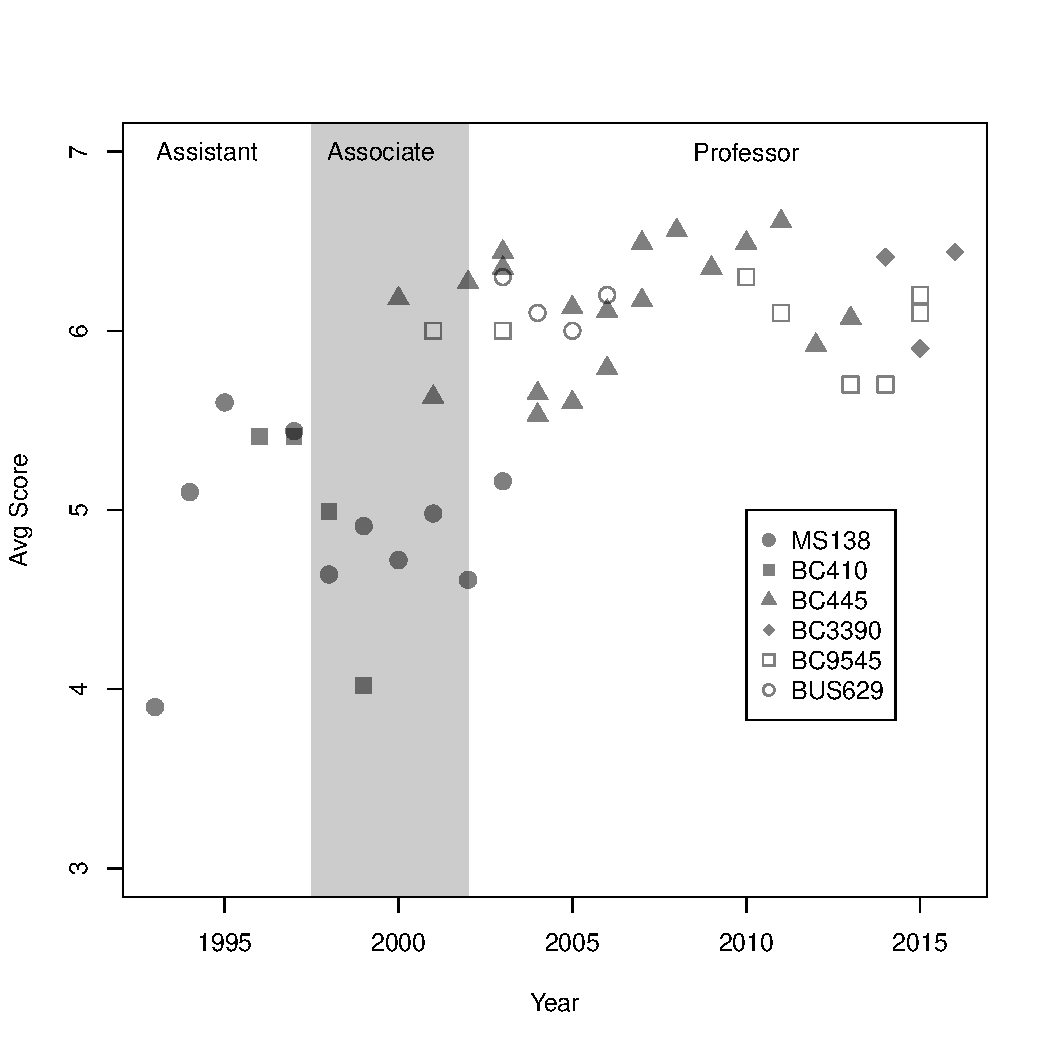
\includegraphics[width=80mm]{data/teaching.pdf}
\label{default}
\end{center}
\end{figure}

I have been involved in teaching all or major portions of seven courses at Western, in addition to the occasional guest lecture. The six main courses are:
\begin{description}
\item{\textbf{MS138:}} (1993-2003) First year medical school introduction to biochemistry. I taught 8-10 lectures that covered nucleotide metabolism, DNA replication and DNA repair as it related to cancer and HIV to first year medical students. I developed the material for delivery, following the broad theme given by the course co-ordinator at the time. The introductory didactic was removed from the undergraduate medical curriculum, along with most basic science, and replaced with small group teaching following a review of the undergraduate medical curriculum. I co-led a basic science review group for this process. I participated in small group teaching for several years afterward, but no evaluations were performed. 
\item{\textbf{BC410:}} (1996-1999) I taught $\frac{1}{3}$ of this course, focussing on the basics of molecular biology pertaining to DNA structure, repair and recombination.  The primary teaching tool was discussion of papers of current research interest with the objective of teaching the scientific discovery process. Included in this was one year of Biochemistry 453, the same course, different number.
\item{\textbf{BC445:}} (2000-2014) I developed and taught this course from scratch, often 2-3x per year. The course broadly covered `bioinformatics' and had a focus on sequence and structure alignment, and at the time of development was rather novel being the first of its kind outside of a computer science department to cover the theory and practice of sequence alignment. The philosophy of the of this course was to teach how sequence alignment algorithms work in an intuitive way. The students would learn how the algorithm worked by doing it by hand, then we would move on to applying computers to make it faster. In addition, students learned the basics of Perl or Awk scripting and how to use a UN*X interface on a computer. Much of this material was rolled into BC3390.   
\item{\textbf{BC3390:}} (2015 - now) A continuation, and simplification of the material in BC445 mandated when the undergraduate Biochemistry department curriculum was revamped.
\item{\textbf{BUS629:}} (2003-2006) I developed and taught this course in the Ivey MBA Biotechnology stream. I was responsible for all the material and for arranging guest experts. The thrust of the course was to teach non-science students in the MBA program how to quickly evaluate the business case for a biotechnology company based on the underlying science. This course was case-based and we discussed one case per week. I wish that Theranos was active at the time --- it would have been a great example of foolish money chasing bad science. I received a citation from the Ivey Dean for teaching excellence.
\item{\textbf{BC9545:}} (2000 - now) This course initially was a more advance presentation of BC445 for graduate students. Since taking the course on compositional data analysis in 2014, I have redesigned it to be a course on the theory and practice of analyzing high throughput sequencing datasets --- transcriptomics and metagenomics. I teach the theory and practice of probabilistic compositional data analysis for such datasets alongside the more traditional methods. My focus is on getting the students to understand and recognize when and why traditional methods go off the rails, and how they can use probabilistic compositional data analysis  to double check their results. 
 \end{description} 

The seventh course was a graduate computer science course. 

\begin{description}
\item{\textbf{CS881:}} (1996 - 2001) “Topics in computing and biology” Graduate Course. Six hours of
lectures on the basics of DNA and on manipulations 	of DNA that could be used for primitive 	computational operations.
\end{description}
\subsection{Summary of HQP}
\begin{description}\itemsep=2pt
\item Graduate Students : 15;  Undergraduate Student: 30; Postdoctoral Fellow: 2; 
\item PhD Thesis Defence Examiner: 37
\item MSc Thesis Defence Examiner: 44
\item Thesis qualifying examiner: 48.
\end{description}

\subsection{Graduate Students Supervised}~

\vspace{0.5cm}
\begin{tabular}{llll}
Year & Student & Role &  Description \\ \hline
2018-IPR & Joris & MSc (BC) & Defining correlated features in microbiomes\\
2017-IPR & Giguere & PhD (BC) & Integrative 'omic analysis  of microbiomes\\
2017 & Giguere & MSc (BC) & Visual exploration of multivariate multi-omic datasets\\
2017 & Gajudhur & MSc (BC) & Visual exploration of multivariate multi-omic datasets\\
2013-2018 & Macklaim & PDF & Microbial community composition of environmental datasets\\
2013-2016 & Wong & MSc (BC) & Microbial community composition of patient cohorts\\
2012-2013 & DiBella & MSc (MI, co) & Role of antisense transcription in bacterial gene regulation\\
2011-2017 & McMurrough & PhD (BC, co) & Coevolution in LAGLIDAG endonucleases\\
2008-2013 & Macklaim & PhD (BC) & Meta-omics of the vaginal microbiome\\
2008-2013 & Dickson & PhD (BC) & Coevolution in protein families\\
2007-2012 & Fernandes & PDF & Statistical tools for microbiome analysis\\
2002-2004 & Gao & MSc (BCE, co) & Cell Surface Expression of Vitreoscilla Hemoglobin \\
2001-2008 & Weedmark & PhD (BC) & DNA repair in Drosophila\\
1998-2005 & Coveny & PhD (BC) & Polycomb genes and DSB\\
1997-1999 & Ding & MSc (BCE, co) & Membrane display of an INP fusion protein\\
1994-1998 & Dray & PhD (BC) & Targeting heterologous sequences in \emph{Drosophila melanogaster}\\
1993-1998 & Keeler & PhD (BC) &  element induced double-strand break repair\\
1993-1995 & Raynor & MSc (BC) & P element excision-induced double strand gap repair \\
1991-1995 & Andrews & MSc (BC)&  KP leucine zipper in the regulation of P transposition\\
\end{tabular} 

\clearpage

\section{Service to the University and Broader Community}

\subsection{University Committees}~

\vspace{0.5cm}
\begin{tabular}{lll}
Year & Role & Description \\ \hline
2016 & Member & Western NSERC Science Review Board\\
2012 & Member & Law Graduate Program Review Committee\\
2011-2014 &  Member & Computer Science Promotion and Tenure Committee\\
2011-2013 &  Member & SUPR-G Committee\\
2011 &  Member & Faculty of Law and Ivey Business School  Joint Promotion and Tenure Committee\\
2005-2006 &  Member & Ivey Business School Promotion and Tenure Committee\\
2005 & Reviewer & External reviewer for Developmental Biology Graduate Program\\
2001-2004 & Member  & Promotion and Tenure - Biology Department\\
2001-2002 & Member & UWO Bioinformatics Tier 2 CRC Search Committee\\
2000-2002 & Member & Senate Subcommittee on Computing and Network Security\\
2000-2003 & Chair & Senate Subcommittee on the WWW (SUWWW)\\
2000-2001 & Member & Accessibility Subcommittee of SUWWW\\
1999-2000 & Member & Biochemical Engineering Chair Selection Committee\\
1998-1999 & Member & Senate Subcommittee on Computing and Network Services\\
1998-1999 & Member & Senate Subcommittee on Computing and Information Technology\\
1997-1999 & Member & Scientific Computing Research Advisory Subcommittee \\
1996-2000 & Member & UWO Homepage Design and Implementation Subcommittee of SUWWW\\
1996-2000 & Member & Senate Subcommittee on the WWW	(SUWWW) \\
1995-2001 & Chair & Molecular Biology Interfaculty Program Steering Committee\\
1995-2001 & Chair & Molecular Biology Interfaculty Program Course Committee\\
1994 & Co-Chair &  Molecular Biology Interfaculty Program Open House\\
1993 & Member & National Scholarship Selection Committee\\
\end{tabular} 

\subsection{Faculty Committees}~

\vspace{0.5cm}
\begin{tabular}{lll}
Year & Role & Description \\ \hline
2010-2013 & Member & Microbiology \& Immunolgy Promotion and Tenure Committee\\
2007-2008 & Member & Epidemiology and Biostatistics Chair Selection Committee\\
2007 & Member & Ad hoc Faculty member disciplinary committee\\
2005-2007 & Chair & Information  Resources Institutional Self Study Task Force\\
2004-2006 & Member & Promotion and Tenure - Pharmacology and Physiology Department\\
2001-2003 & Member & Human Molecular Genetics Selection Committee\\
1999-2000 & Chair & Information  Resources Institutional Self Study Task Force\\
1997-2001 & Member & UMEC Appeals Committee\\
1996-1998 & Member & Medical Science Building Study Group\\
1996-1999 & Member & Molecular Genetics Task Force\\
1996-1999 & Co-Chair & Life Sciences group for the Medical School Curriculum renewal process\\
1996-2001 & Member & ACMC Medical Informatics Group\\
1995-1996 & Member & Computer and WWW Task Force\\
1994-2001 & Member & Dean's advisory Committee on Genetics\\

\end{tabular} 

\vspace{0.5cm}
\subsection{Department Committees}~

\vspace{0.5cm}
\begin{tabular}{lll}
Year & Role & Description \\ \hline
2019-present Chair, Department of Biochemistry
2015-2017 & Member (Seconded) & Biochemistry Promotion and Tenure Committee\\
2012-2015 & Member & Research Committee	\\
2010-2013 & Member & Undergraduate Committee\\
2009-2012 & Member & Biochemistry Promotion and Tenure Committee\\
2009-2012 & Member & Appointments Committee\\
2004-2008 & Chair & Biochemistry Graduate Studies\\
2002-2004 & Member & Biochemistry Graduate Studies\\
2001-2004 & Chair & Visiting Speakers Committee\\
1998-2004 & CoChair & Department Outreach Committee\\
1997 &  Member & Biochemistry Promotion and Tenure Committee\\
1996 & Chair & Nominating Committee\\
1995-2005 & Member & Ad hoc  Computing Advisory Committee\\
1995-1998 & Member & Area, Safety, Equipment and Animal Care Committee\\
1993-1996 & Member & Nominating Committee\\
1993-1996 & Member & Graduate Studies Committee\\
\end{tabular} 

\subsection{Board memberships}
\begin{description}
\item 2001-2002,	Member, Board of Directors for Partners in Research
\item 1995-2001	Member, Board of Directors, The Foundation for Gene 	and Cell Therapy (FFGCT).\\ I was the lead negotiator for 	the FFGCT in working out a partnership with the MRC 	to fund up to 9 post-doctoral fellows in the area of gene 	therapy. This partnership provided approximately 	\$900,000 in new money to the MRC.
\item 1995,	Member of the Home Team for Jesse’s Journey 	(Internet and Science Advisor).\\ I posted and updated a 	World Wide Web map page so that people from around the 	world could follow John and Jesse’s progress.
\end{description}

\subsection{Grants and Awards Panels, Editorial membership, External Committees}

\begin{description}\itemsep=2pt
\item 2019-2021, Member, CodaWorks Meetings Committee 
\item 2016-present, Chair, CIHR Project Grant Scheme (GMX committee)
\item 2017-present, Member, CIHR College of Reviewers (First round invitee)
\item 2017, Member, Canadian Crohns and Colitis Review panel
\item 2016, Member, Agence Nationale de la Recherche, Preindustrial Biotechnology Demonstrator, Paris, France
\item 2018-2019, Associate Editor, Microbiome
\item 2016-2018, Section Editor, Microbiome
\item 2016, Western Science and Engineering Review Board Member
\item 2016, CIHR Operating Grant Review Panel Chair
\item 2015-2016, Associate Editor, Microbiome
\item 2015, Ontario Genomics Institute: Large Scale Applied Research Program review panel
\item 2014-present, CRC College of Reviewers
\item 2012-2015,	Editorial Board member Microbiome
\item 2010-2014,	Member CIHR Genetics panel 
\item 2008-present,	IODE Doctoral Scholarship committee 
\item 2006-2010, 	NCIC Model Organisms Panel B2 
\item 1998, 1999, 2000, 2003, 2004, 2005, 2006, 2007, 2008 MRC/CIHR BMB/Genetics/Genomics invitee
\item 1999, 		Chair OGS Biochemistry/Biophysics panel 
\\item 1997-1999,  	OGS Biochemistry/Biophysics panel 
\item 1997–2000, 	NCIC Virology and Molecular Biology Committee\\ Panel F
\item  1995-2001, Foundation for Gene and Cell Therapy (Jesse's Journey)\\ Chair and Review Organizer 1995 - 2001
\end{description}

\end{document}